%%%%%%%%%%%%%%%%%%%%%%%%%%%%%%%%%%%%%%%%%%%%%%%%%%%%%%%%%%%%%%%%%%%%%%
%% all the formatting stuff and packages

\documentclass[11pt]{article}

\parindent0em
\parskip.5em

\usepackage{xstring}

\usepackage{amsthm}
\usepackage[utf8]{inputenc}
\usepackage[ttscale=.85]{libertine}
\usepackage{libertinust1math}
% \usepackage[libertine,cmintegrals,cmbraces,vvarbb]{newtxmath}
\usepackage[T1]{fontenc}
\usepackage{microtype}
\usepackage{amsmath}
\usepackage{amssymb}
\usepackage{xspace}
\usepackage{ngerman}
\usepackage{graphicx}
\usepackage{lastpage}
\usepackage{ifthen}
\usepackage{fp}
\usepackage{hyperref}
\usepackage{icomma}
\usepackage{paralist}
\usepackage[ngerman,onelanguage,noend]{algorithm2e}
\DontPrintSemicolon

\makeatletter
\DeclareRobustCommand{\bfseries}{%
   \not@math@alphabet\bfseries\mathbf
   \fontseries\bfdefault\selectfont
   \boldmath
}
\makeatother

\usepackage[headsep=1cm]{geometry}

\usepackage{fancyhdr}

\fancypagestyle{plain}{%
  \renewcommand{\headrulewidth}{0pt}%
  \fancyhf{}
  \rhead{
\includegraphics[width = 2.4cm]{fig/hpi_logo.pdf}}
  \lhead{\textbf{\sffamily Parametrisierte Algorithmen} \\
    \textbf{\sffamily Wintersemester 2017/2018} \\
    \sffamily Thomas Bläsius}
  \cfoot{\thepage}
  \rfoot{\ifthenelse{\thepage < \pageref{LastPage}}{\textit{bitte
        wenden}}{}}
}
\fancypagestyle{normal}{%
  \renewcommand{\headrulewidth}{0pt}%
  \fancyhf{}
  \cfoot{\thepage}
  \rfoot{\ifthenelse{\isodd{\thepage} \and \thepage <
      \pageref{LastPage}}{\textit{bitte wenden}}{}}
}

\usepackage{titlesec}

\titleformat{\section}%
[hang]%
{\Large\bfseries\sffamily}%
{Aufgabe \thesection:}%
{.5em}%
{}%
[]

\renewcommand{\thesubsection}{\alph{subsection}}
\usepackage{titlesec}
\titleformat{\subsection}%
[runin]%
{\bfseries\sffamily}%
{Teilaufgabe (\thesubsection)}%
{0pt}%
{}%
[]

\usepackage{titlesec}
\titleformat{\subsubsection}%
[hang]%
{\large\bfseries\sffamily}%
{\thesection}%
{.5em}%
{}%
[]

\titlespacing{\section}{0pt}{1.5ex}{.5ex}

\titlespacing{\subsection}{0pt}{.5ex}{.5em}

\titlespacing{\subsubsection}{0pt}{1ex}{.5ex}


%%%%%%%%%%%%%%%%%%%%%%%%%%%%%%%%%%%%%%%%%%%%%%%%%%%%%%%%%%%%%%%%%%%%%%
%% commands to use in the exercise sheet/solution

\newcommand{\sheet}[2]{ %
  \title{\textbf{\sffamily Übungsblatt #1}\\[-0.5ex]
    {\normalsize \sffamily Abgabe bis #2}}
  \date{}
  \maketitle
  \pagestyle{normal}
  \vspace{-2cm}
}

\newcommand{\solution}[2]{ %
  \title{\textbf{\sffamily Musterlösung zum Übungsblatt #1}\\[-0.5ex]
    {\normalsize \sffamily Erstellt von #2}}
  \date{}
  \maketitle
  \pagestyle{normal}
  \vspace{-2cm}
}

\newcommand{\exercise}[2][]{%
  \section{#2 \hfill {\normalsize#1}}%
}

\newcommand{\subexercise}{%
  \subsection{}%
}

\newcommand{\how}[1]{%
  \subsubsection*{Wie kommt man drauf?}%
}




\DeclareMathOperator{\vc}{vc}

\begin{document}

\solution{2}{Marvin Mirtschin, Tobias Stengel und Sören Tietböhl}

\exercise{Punkte und Geraden}

Zunächst wird das Problem unter Verwendung der folgenden Reduktionsregel auf einen Kern reduziert:

\textbf{Reduktionsregel 1:}
\begin{itemize}
\item suche eine Gerade $g$, die mindestens $k+1$ Punkte abdeckt und füge $g$ zur \mbox{\textsc{Geradenüberdeckung}} hinzu
\item lösche alle von $g$ abgedeckten Punkte aus $P$ und reduziere $k$ um 1
\end{itemize}
Diese Reduktionsregel ist sicher. Angenommen die Instanz $I$ sei gegeben und $I$ sei vor der Reduktion lösbar. Würde man $g$ nicht zur \textsc{Geradenüberdeckung} hinzufügen, müsste man jeden der Punkte, die von $g$ abgedeckt werden, durch eine eigene Gerade abdecken. Da $g$ mindestens $k+1$ Punkte abdeckt, würden dafür alleine also wenigstens $k+1$ Geraden benötigt werden, die Größe der \textsc{Geradenüberdeckung} könnte also nicht mehr eine Größe ${\leq}k$ haben.

Diese Regel wird solange angewendet, wie möglich. Beinhaltet der danach verbleibende Kern mehr als $k^2$ Knoten, ist keine \textsc{Geradenüberdeckung} mit maximal $k$ Geraden mehr möglich. Grund dafür ist, dass mit den verbleibenden $k$ Geraden je maximal $k$ Punkte abgedeckt werden (sonst könnte Reduktionsregel 1 erneut angewendet werden). Insgesamt können mit den $k$ verbleibenden Geraden also maximal $k^2$ Punkte abgedeckt werden.

Dieses Kernproblem der Größe $O(k^2)$ kann nun mittels Brute-Force gelöst werden.

Für den Test, ob es eine Gerade $g$ gibt, die mindestens $k+1$ Punkte abdeckt, wird für jedes Paar von Punkten ($O(n^2)$) geprüft wie viele Punkte die Gerade, die diese beiden Punkte verbindet, abdeckt. Dafür muss potentiell pro Gerade für jeden der verbleibenden $n-2$ Punkte entschieden werden, ob er auf der Gerade liegt oder nicht. Falls er auf der Geraden liegt, wird der Wert, der sich merkt, wie viele Punkte auf einer Geraden liegen, inkrementiert. Ein Reduktionsschritt liegt damit in $O(n^3)$.

Die Reduktionsregel wird maximal $k$ mal angewendet, da nach jeder Anwendung $k$ um 1 reduziert wird. Falls $k$ auf 0 fällt, hat man die \textsc{Geradenüberdeckung} gefunden, falls kein Knoten mehr übrig bleibt. Die Kernbildung liegt also insgesamt in $O(k*n^3)$, und da $k{\leq}n$ gilt, liegt sie insbesondere in $O(n^4)$.

Das Kernproblem wird mittels Brute-Force gelöst. Dafür werden zunächst alle möglichen Geraden gebildet, indem jedes Knotenpaar eine Gerade darstellt. Da es maximal noch $k^2$ Knoten gibt, liegt die Anzahl der Geraden in $O(k^4)$. Für jede dieser Geraden kann (wie bereits oben beschrieben) wieder überprüft werden, welche Punkte auf ihr liegen. Neben der Anzahl der abgedeckten Punkte ist hier vor allem interessant, welche Punkte genau abgedeckt werden. Dazu kann pro Gerade eine Bitmap der Größe $=k^2$ gespeichert werden, die mit 1 markiert wird, wenn ein Punkt von der Gerade abgedeckt wird. Das Erstellen einer Bitmap liegt in $O(k^2)$, da jeder Punkt geprüft wird. Da es $k^4$ Geraden gibt, liegt die Erzeugung aller Bitmaps in $O(k^6)$. Nun wird für jede Teilmenge aller Geraden geprüft, ob diese Teilmenge alle verbleibenden Punkte abdeckt. Insgesamt gibt es potentiell $2^{k^4}$ Teilmengen. Der Test, ob nun alle Punkte abgedeckt werden kann mithilfe der Bitmaps in $O(k^3)$ erledigt werden, da pro Bitmap maximal $k^2$ Werte gespeichert werden und maximal $k$ Geraden noch verwendet werden können. Der gesamte Brute-Froce Schritt liegt damit in $O(k^6+k^3*2^{k^4})$.

Der gesamte Algorithmus liegt damit in $O(k^6+k^3*2^{k^4}+n^4)$ und ist damit $\in FPT$.

\exercise{Dominierende Mengen}

Wir gehen dabei ähnlich vor, wie beim FPT-Algorithmus für Independent Set aus der Vorlesung.

Wir nehmen an, dass die Aufgabenstellung nur wissen möchte, ob es ein Connected Dominating Set der Größe $k$ gibt. Weiterhin nehmen wir an, dass wir nur Zusammenhängende Graphen betrachten.
Diese Eigenschaft können wir leicht in $\Theta(m)$ mit einer Breitensuche sicherstellen.
Die Baumzerlegung ist als schöne Baumzerlegung vorliegend.

Der einzige Unterschied zum Algorithmus aus der Vorlesung besteht darin, wie wir die Regeln für Introduce, Forget und Join Knoten wählen.

Für Introduce Regeln gehen wir wie folgt vor (Beispiel von Folie 4, 3.Vorlesung):

\begin{center}
\begin{tabular}{c c c c c c c c}
    $\emptyset$ & $\{4\}$ & $\{5\}$ & $\{6\}$ & $\{4,5\}$ &$\{4,6\}$ &$\{5,6\}$ &$\{4,5,6\}$\\
    $\infty$ & 2 & 2 & $\infty$ & 3 & 3 & 3 & 4\\
\end{tabular}
\end{center}

wird zu

\begin{center}
\begin{tabular}{c c c c}
    $\emptyset$ & $\{4\}$ & $\{6\}$ & $\{4,6\}$\\
    $\infty$ & 2 & 3 & 3\\
\end{tabular}
\end{center}

wobei sich der Eintrag für 4 aus dem Minimum von $\{4\}$ und $\{4,5\}$,
für 6 aus dem Minimum von $\{6\}$ und $\{5,6\}$, sowie für $\{4,6\}$ aus dem Minimum von $\{4,6\}$ und $\{4,5,6\}$ berechnet.
Der Eintrag für $\emptyset$ kommt von $\{6\}$.

Für introduce Knoten gehen wir wie folgt vor:

\begin{center}
\begin{tabular}{c c c c}
    $\emptyset$ & $\{4\}$ & $\{6\}$ & $\{4,6\}$\\
    $\infty$ & 2 & 3 & 3\\
\end{tabular}
\end{center}

wird nach Hinzufügen von $\{7\}$ zu

\begin{center}
\begin{tabular}{c c c c c c c c}
    $\emptyset$ & $\{4\}$ & $\{7\}$ & $\{6\}$ & $\{4,7\}$ &$\{4,6\}$ &$\{7,6\}$ &$\{4,7,6\}$\\
    $\infty$ & 2 & $\infty$ & $\infty$ & 3 & 3 & $\infty$ & 4\\
\end{tabular}
\end{center}

Da 7 keine Verbindung zu 6 hat, kann also 6 oder 7 alleine nicht funktionieren. Auch $\{7,6\}$ kann nicht funktionieren, da 4 7 vom Rest separiert. ($\{4,6\}$ ist ein Seperator für 7)

Ein Sonderfall kann noch auftreten, dafür Betrachten wir den grünen Teil des Graphen auf Folien 8 und 9 , Vorlesung 3.
Beim Schritt von $\{U,n\}$ zu $\{U,5,n\}$ tritt der Fall ein, dass weder $U$ noch $n$ mit 5 verbunden sind. Nach der obigen Berechnung würde dann überall $\infty$ stehen.
Damit die Ergebnisse brauchbar bleiben, ignorieren wir hier die \emph{Connected}-Eigenschaft und berechnen nur ein Dominating Set. Wir tun also so, als ob 5 mit beiden anderen Knoten verbunden wäre und berechnen die Werte entsprechend.
Das Ganze funktioniert deshalb, weil 5 anschließend mit einem anderen Strang verjoined wird, welcher 5 mit einem der anderen Knoten verbinden kann.

Solch ein Join Knoten muss in der schönen Baumzerlegung immer existieren, da der Graph zusammenhängend ist.
Betrachten wir den Fall, dass ein Knoten $x$ introduced wird, der keine Verbindung zu den Knoten in seinem Bag $B = \{x, b_1, \dots , b_n\}$ hat.
Dann muss es einen Pfad $\{x, k_1, \dots, k_i, b_k\}$ geben, der $x$ mit einem der Knoten aus $B$ verbindet (weil der Graph zusammenhängend ist).

Die Knoten $\{k_1, \dots, k_i\}$ können bisher in keinem Unterknoten von $B$ aufgetaucht sein, da $B$ ein Seperator ist. Falls einer der Knoten aufgetaucht wäre, könnten nicht mehr alle Verbindungen durch Bags abgedeckt werden, da $x$ grade introduced wurde. (Und in einer schönen Baumzerlegung wird jeder Knoten auf dem Pfad zur Wurzel max 1 mal introduced)

D.h. es muss noch einen zweiten Ast des Baumes geben, auf dem dann die Knoten des Pfades abgearbeitet werden. Dort befinden sich dann auch $x$ und $b_k$ irgendwann in einem Bag. Damit die Teilbaum Eigenschaft erhalten bleibt müssen $x$ und $b_k$ also an einem Join beteiligt sein. Demnach werden $B$ und $B_2$ bzw darüberliegende Bags verjoined.

Bleibt also nur noch die Vorgehensweise eines Joins zu beschreiben. Das passiert identisch zum Algorithmus aus der Vorlesung.
D.h. der neue Wert einer Menge berechnet sich aus der Addition der alten Werte minus der Kardinalität.

\exercise{Baumweite planarer Graphen}

Die Grundidee besteht darin, das Planar Seprarator Theorem rekursiv anzuwenden, um den Graph in immer kleinere Teile zu zerteilen, bis die Teile alle kleiner als $\sqrt{n}$ sind.

Z.B. nach 2-maliger Rekursion:

\begin{center}
    \vspace{1ex}
    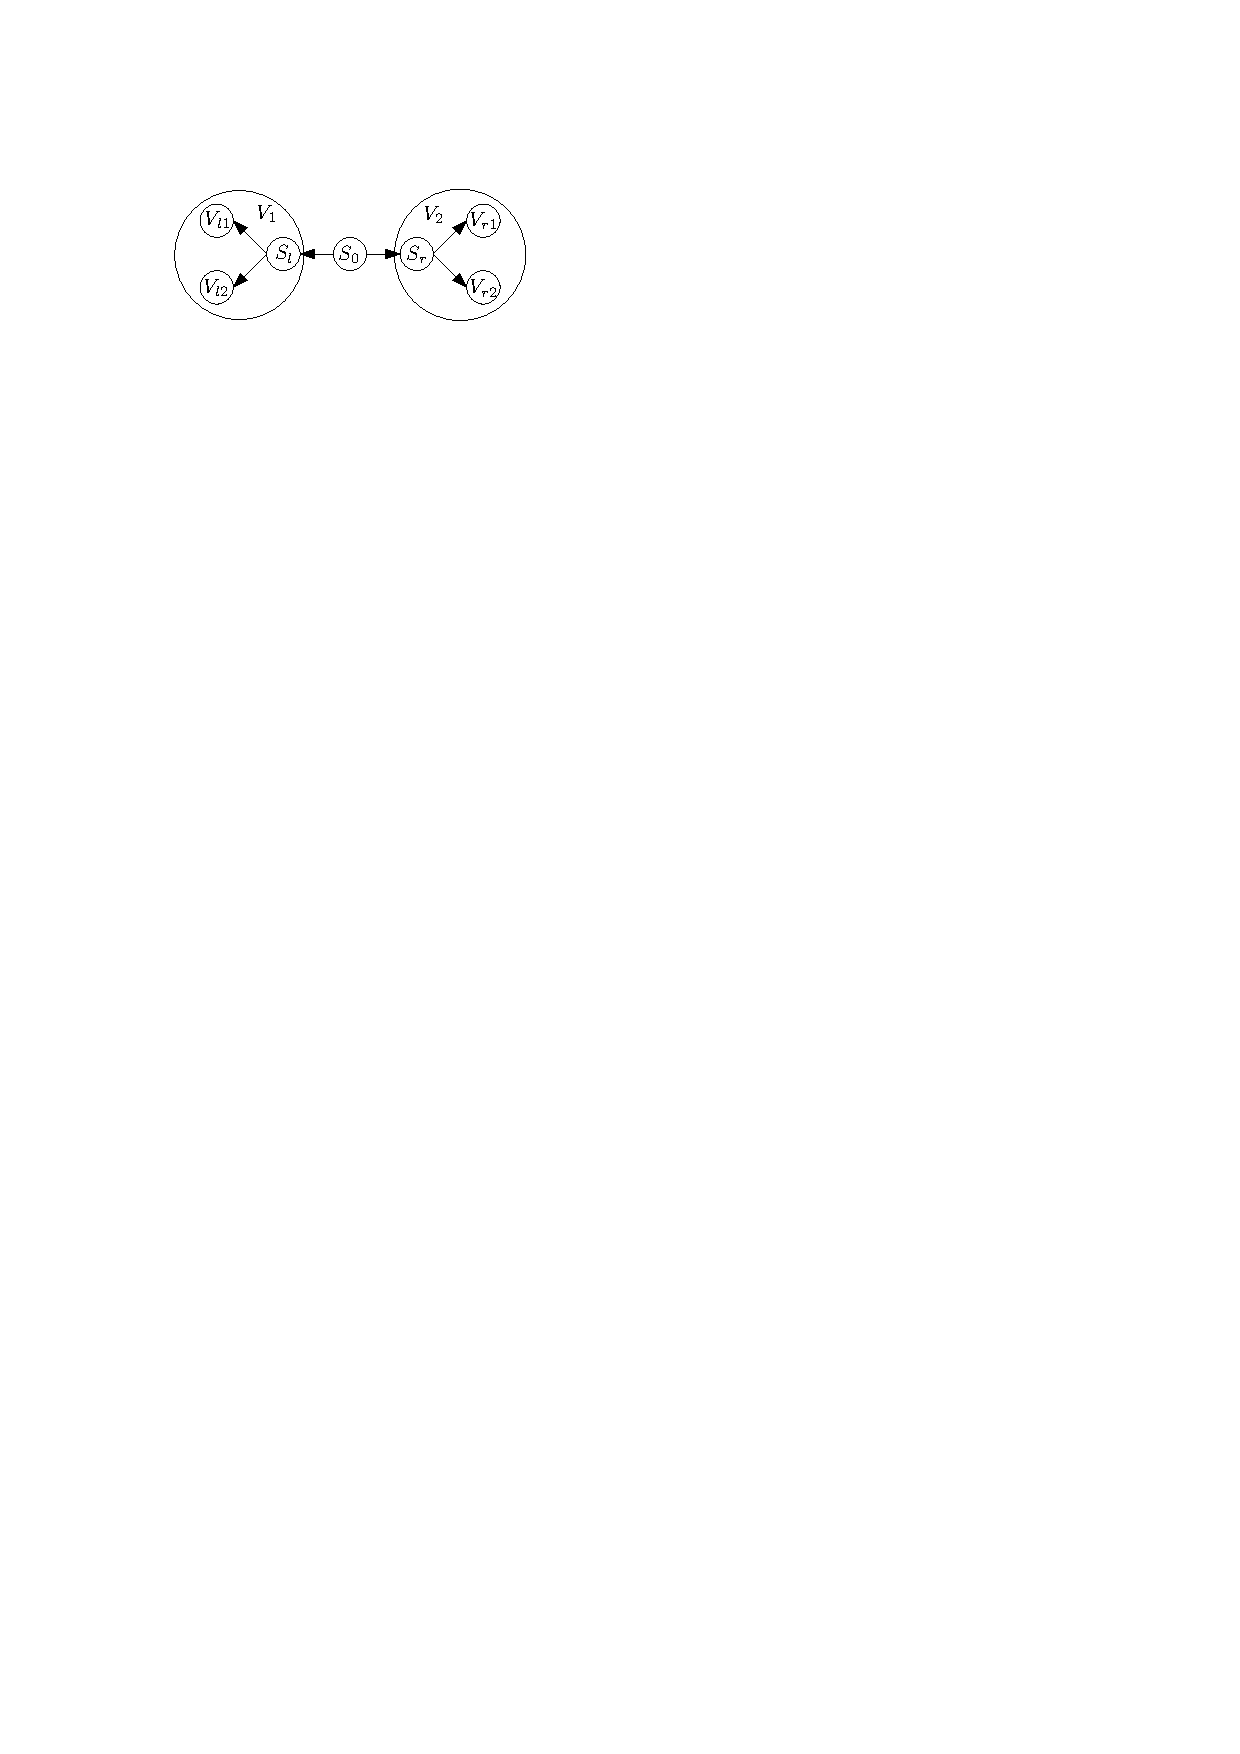
\includegraphics[page=1]{fig/02-A3}
  \end{center}

Dabei hat nach Aussage des Theorems die Menge $S_0$ die Größe $|S_0| \leq 4\sqrt{n}$, sowie $|S_l|,|S_r| \leq 4\sqrt{\frac{2}{3}n}$
Wenn wir nun einfach alle $S_i$ zu eigenen Bags machen, haben wir schon fast eine Baumzerlegung, die Baumweite in $\Theta(\sqrt{n})$ hat.
Wir müssen nur noch die Eigenschaft erfüllen, dass Knoten die Kanten zueinander haben auch zusammen in einem Bag auftauchen. Das ist momentan noch nicht gegeben, da die Seperatoren i.Allg. mit den jeweiligen $V_k$ verbunden sind.

Dazu schauen wir uns einmal in unserem oberen Graphen einen Pfad von einem $S_i$ zur Wurzel $S_0$ an. Sei der Pfad als $\{S_i, S_{i-1}, \dots, S_0\}$ gegeben.
Wir wählen dann das entsprechende Bag für $S_k$ als $B_k = \bigcup\limits_{i=0}^k S_i$. Dabei setzen wir die Bags für $S_{kl}$ und $S_{kr}$ als Kinder des Bags $B_k$, sowie das Bag $B_k$ als Kind von $B_{k-1}$.
Die Größe des Bags $B_k$ berechnet sich als
$$ |B_k| = \sum\limits_{i=0}^k |S_k| = \sum\limits_{i=0}^k \left(4\sqrt{n}\sqrt{\frac{2}{3}^i}\right) = 4\sqrt{n}\sum\limits_{i=0}^k \sqrt{\frac{2}{3}^i}$$

$$ \sum\limits_{i=0}^k \sqrt{\frac{2}{3}^i} \leq \sum\limits_{i=0}^{\infty} \sqrt{\frac{2}{3}^i} = \frac{1}{1 - \frac{1}{3}} = \frac{3}{2}$$

$$ 4\sqrt{n}\sum\limits_{i=0}^k \sqrt{\frac{2}{3}^i} \leq 4\sqrt{n} \frac{3}{2} = 6\sqrt{n}$$

$\Rightarrow B_k \leq 6\sqrt{n}$ für alle $k$

Mit dieser Wahl der Bags können wir nun garantieren, dass es für jedes verbundene Knotenpaar ein Bag gibt in dem beide Knoten auftauchen.
Das liegt daran, dass jeder Knoten aus $V_l$ bzw $V_r$ in einem Bag landet, welches alle Knoten aus $S$ und den Vorgängern von $S$ beinhaltet. Knoten aus $V_l, V_r$ haben nur interne Verbindungen oder Verbindungen zu $S$ oder den Vorgängern von $S$, sonst nirgends anders hin - so haben wir die Seperatoren schließlich gewählt.

Also haben wir nun eine Baumzerlegung, die alle Knoten abdeckt, bei der verbundene Knoten zusammen in einem Bag auftauchen und bei dem die Bags eines Knotens einen Teilbaum ergeben. Letzteres folgt daraus, dass wir Knoten auf dem Weg zu den Blättern nur zu Bags hinzufügen und die vorige Eigenschaft erfüllt ist.

Die Baumzerlegung ist damit gültig und hat eine Baumweite in $\Theta(\sqrt{n})$
\end{document}